\documentclass[12pt]{article}
\usepackage[a4paper, text={17cm,24cm}, top=3cm, left=2cm]{geometry}
\usepackage[utf8]{inputenc}
\usepackage{times}
\usepackage[czech]{babel}
\usepackage[unicode]{hyperref}
\usepackage{graphicx}
\begin{document}

\begin{titlepage}
	\begin{center}

		
\includegraphics[height = 96pt]{img/FIT_barevne_CMYK_CZ.pdf} \\

		\begin{LARGE}
			\textbf{Vysoké učení technické v Brně} \\
		\end{LARGE}

		\begin{large}
			Fakulta informačních technologií \\
			Praktické aspekty vývoje software \\
			2018~/~2019 
		\end{large}
		\\[78mm]

		\begin{huge}
				\textbf{Profilování} \\
			\begin{large}		
		Radim Lipka xlipka02@stud.fit.vutbr.cz
		
        Roman Ondráček xondra58@stud.fit.vutbr.cz
        
        Pavel Raur xraurp00@stud.fit.vutbr.cz
        
        David Reinhart xreinh00@stud.fit.vutbr.cz
        \end{large}
		\end{huge}
	\end{center}

	\vfill


\end{titlepage}

\newpage

\section{Výstupy z profilování}
Pro profilování jsme použili program KCachegrind.
\subsection{Výstupy}
První obrázek pro každou hodnotu vstupu je graf volání z rootu, druhý je pak graf volání z mainu programu.

\noindent Graf volání při spuštění programu s deseti čísly na vstupu:

\begin{figure}[ht]
    \centering
    \scalebox{0.59}{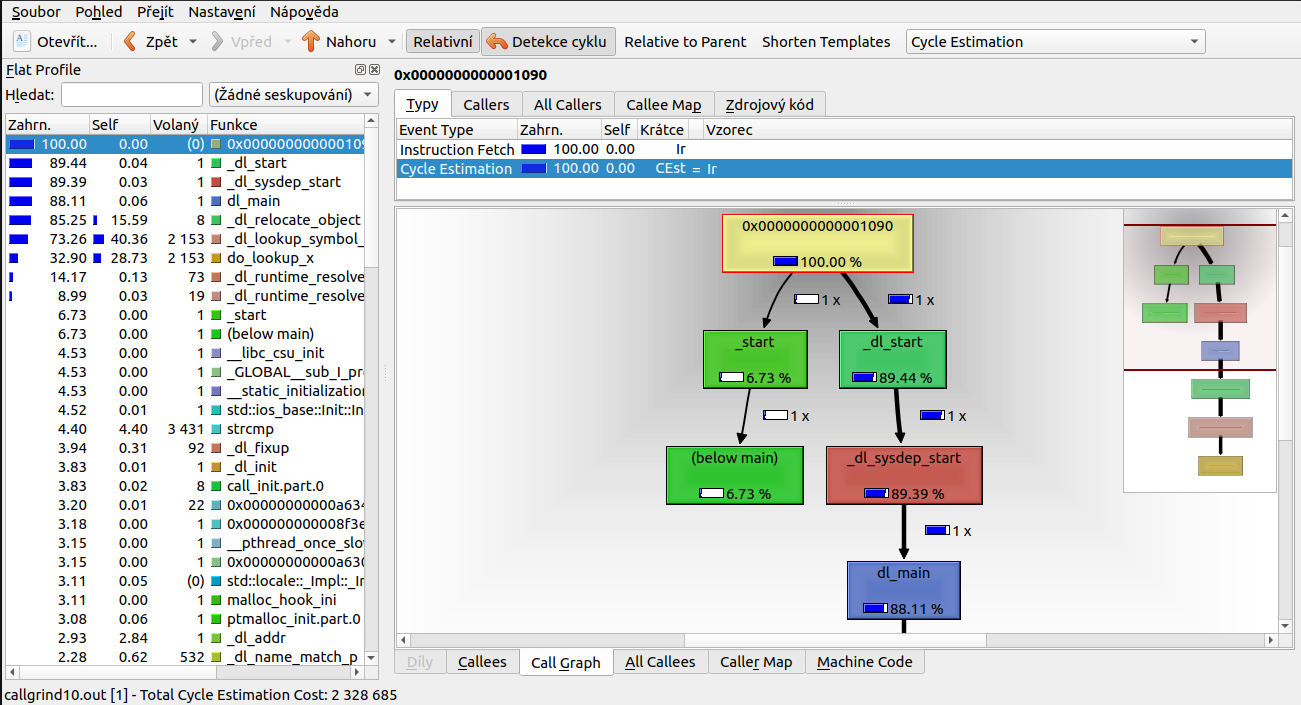
\includegraphics{img/root10.png}}
\end{figure}
\begin{figure}[ht]
    \centering
    \scalebox{0.59}{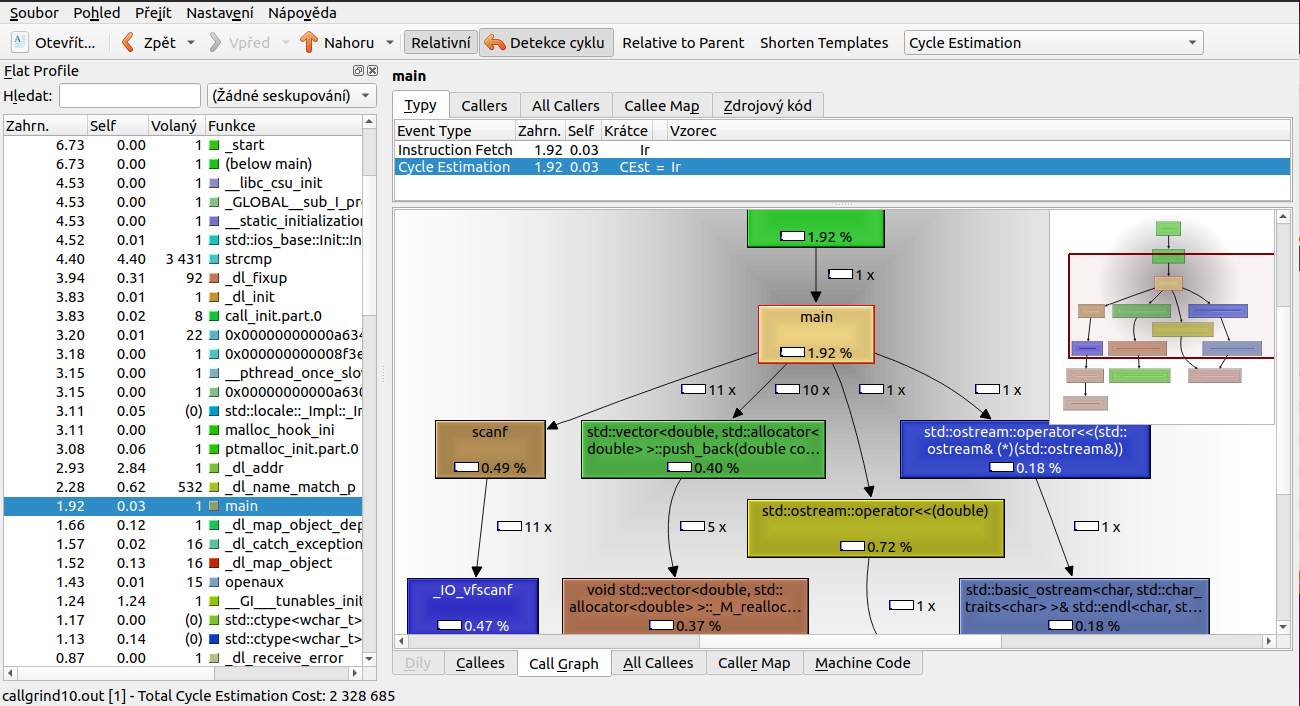
\includegraphics{img/main10.png}}
\end{figure}
\newpage
\noindent Graf volání při spuštění programu se sto čísly na vstupu:

\begin{figure}[ht]
    \centering
    \scalebox{0.59}{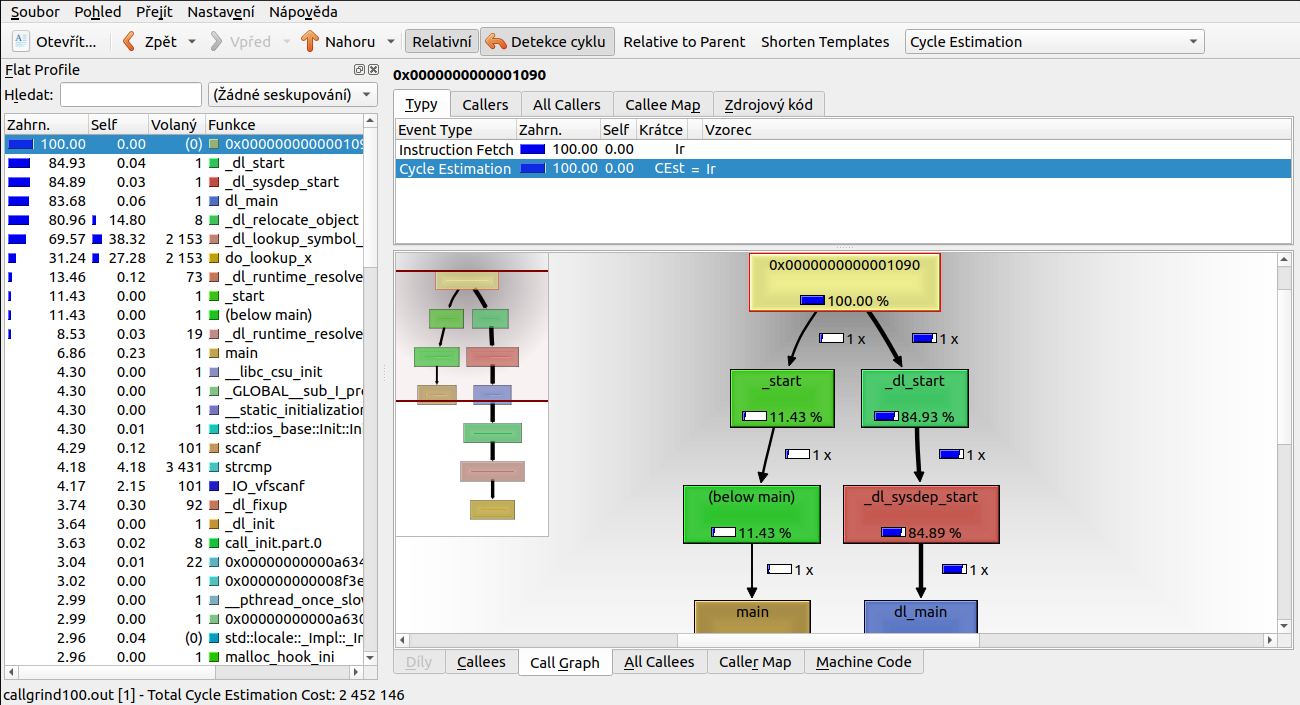
\includegraphics{img/root100.png}}
\end{figure}
\begin{figure}[ht]
    \centering
    \scalebox{0.59}{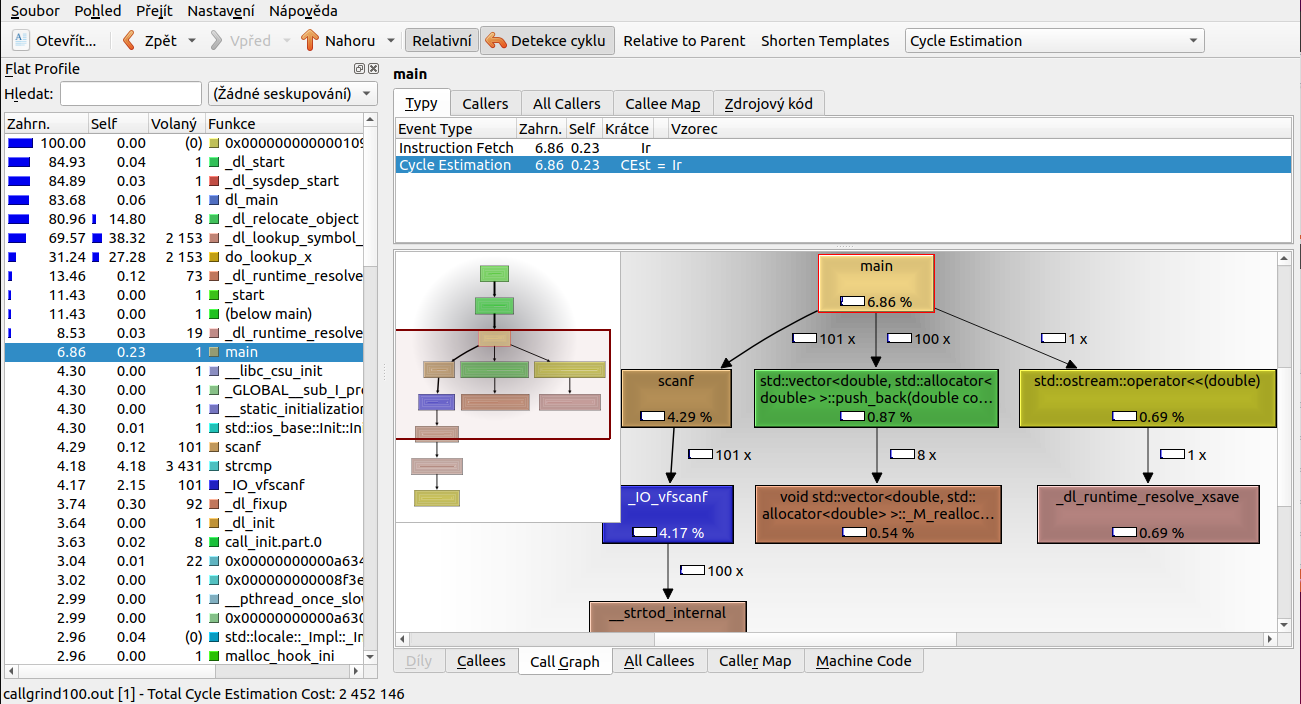
\includegraphics{img/main100.png}}
\end{figure}
\newpage
\noindent Graf volání při spuštění programu s tisíci čísly na vstupu:

\begin{figure}[ht]
    \centering
    \scalebox{0.59}{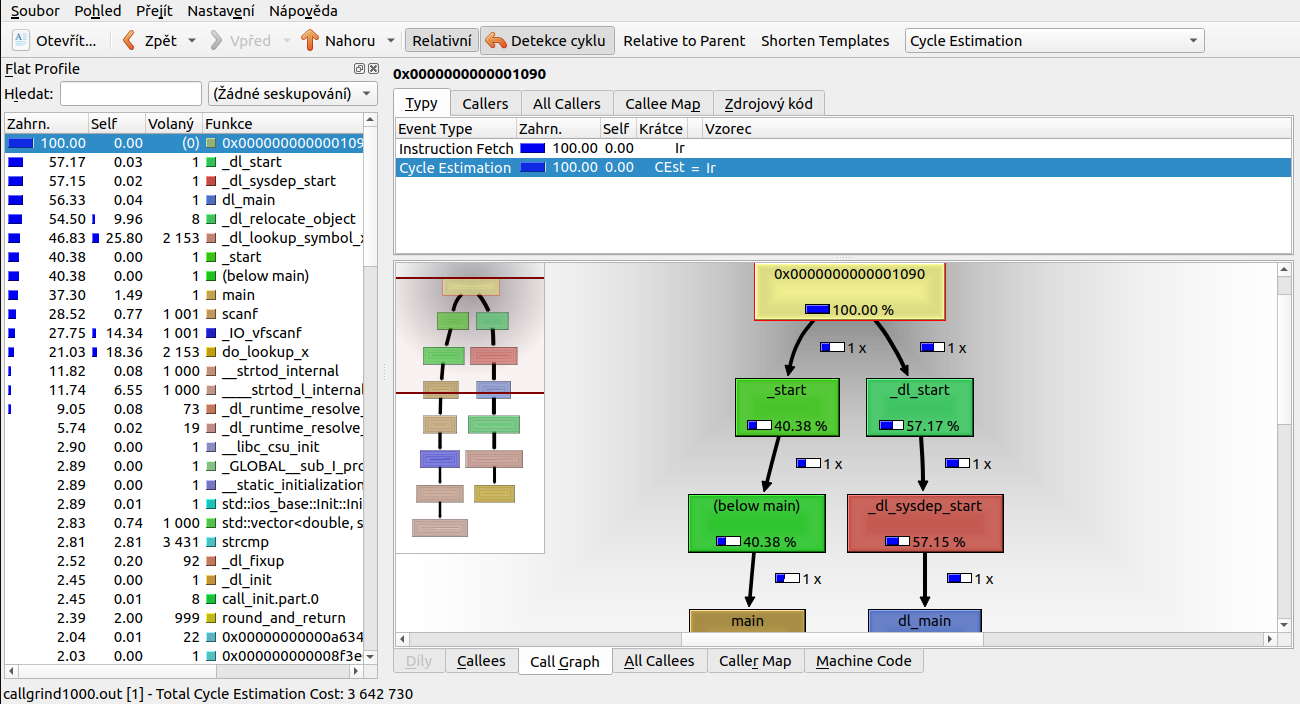
\includegraphics{img/root1000.png}}
\end{figure}
\begin{figure}[ht]
    \centering
    \scalebox{0.59}{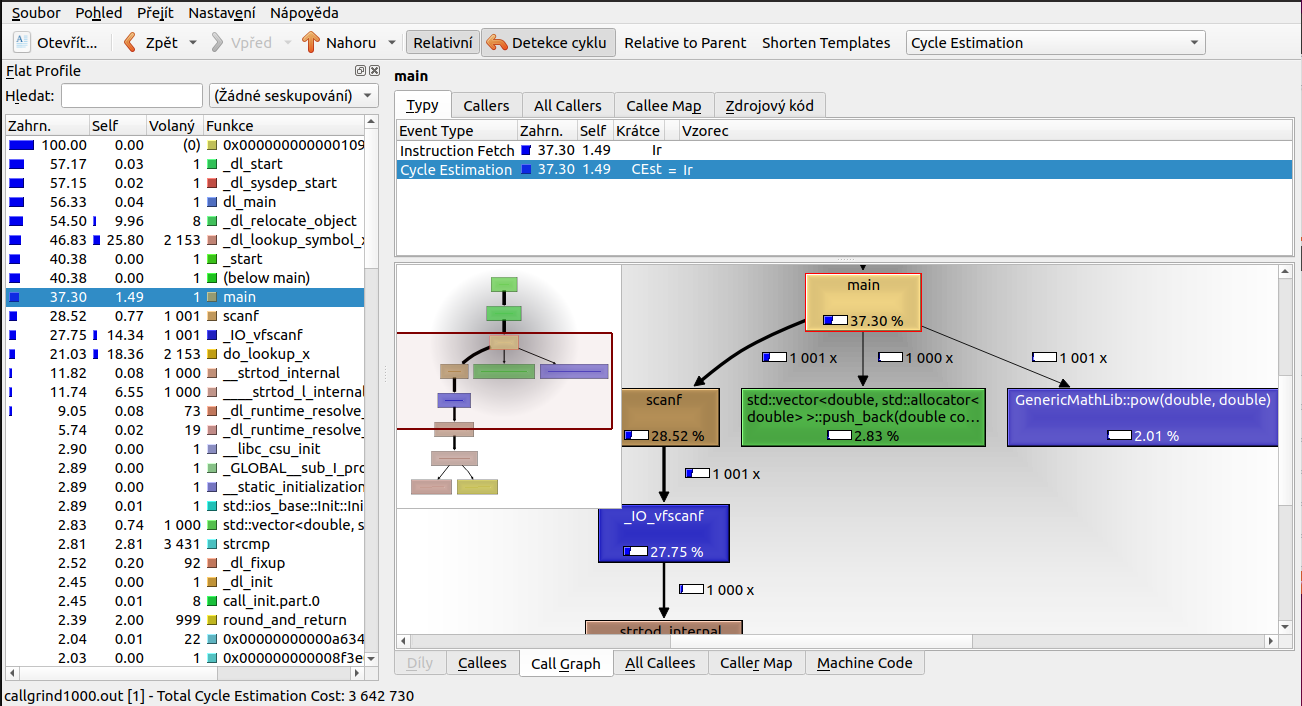
\includegraphics{img/main1000.png}}
\end{figure}
\newpage
\subsection{Shrnutí}
Na všech třech grafech volání, které jsou zobrazeny z kořene je vidět, že úplně nejvíce času tráví program na načítání \textbf {dynamických knihoven}.

\noindent Pokud se podíváme na grafy volání zobrazené z mainu daného programu, můžeme vidět, že v mainu trvá nejdéle provedení funkce \textbf{scanf}.
\subsection{Na co se zaměřit při optimalizacích}
Z těchto výstupů vyplývá, že nejlépe je zaměřit se na způsob sestavování programu a zamyslet se nad tím, zda-li není lepší použít \textbf{statické sestavení knihoven}, které se volají při sestavování programu než \textbf{dynamické sestavení knihoven}, které se volají až při spuštění programu, což daný program zpomaluje a co nejvíce omezit volání různých knihovních funkcí v rozsáhlých cyklech.

\end{document}